\documentclass{article}

\usepackage[utf8]{inputenc}
\usepackage[T1]{fontenc}
\usepackage{geometry}
\usepackage{graphicx}
\usepackage{subcaption}
\geometry{a4paper}

\usepackage[french,italian]{babel}
\frenchspacing

\title{Relazione dell'esperimento di misura della velocità della luce}
\author{Lorenzo Ramella, Alessandro Matteo Rossi, Marco Tambini}
\date{\today}

\begin{document}
\maketitle

\begin{abstract}
L’esperimento si propone di misurare la velocità delle luce usando il metodo di Focault. 
\end{abstract}
\tableofcontents

\section{Introduzione teorica}
Il metodo di Focault per la misura della velocità della luce consiste nell'uso di uno specchio rotante, che riflette la luce emessa da una sorgente su di uno specchio concavo. 

Una sorgente luminosa $S$ emette una luce che, opportunamente diaframmata da una lente $L_1$, attraversa una lastra semitrasparente angolata di 45° rispetto alla direzione del fascio. Una lente $L_2$ focalizza il fascio nel punto $S'$ sullo specchio concavo, dopo essere stata deflessa dallo specchio rotante. La luce riflessa dallo specchio concavo viene deflessa nuovamente dallo specchio rotante, che nel frattempo ha ruotato di un angolo 

\[\alpha = \omega \frac{2D}{c}\]

dove $\omega$ è la velocità angolare dello specchio e $D$ è la distanza tra lo specchio rotante e lo specchio concavo.

Il fascio luminoso di ritorno sulla lente $L_2$ viene focalizzato come se provenisse da una sorgente $S''$ spostata da $S'$ di una quantità 

\[\Delta = 2 \alpha D\] 

Tenendo presente che il fattore di amplificazione $G$ della lente $L_2$ è esprimibile mediante la seguente relazione:

\[G=\frac{b}{D+a}\]

dove $b$ è la distanza tra $L_2$ e la sorgente luminosa e $a$  la distanza tra $L_2$ e lo specchio rotante. Lo spostamento laterale $\delta$ dell'immagine è quindi:

\[\delta = G\Delta =\frac{2\alpha b D}{D + a}=\frac{4 D^2 b \omega}{c(D+a)}\]

\section{Progettazione dell'esperimento}

\begin{figure}[h]
  \centering
  \begin{subfigure}[b]{0.4\linewidth}
    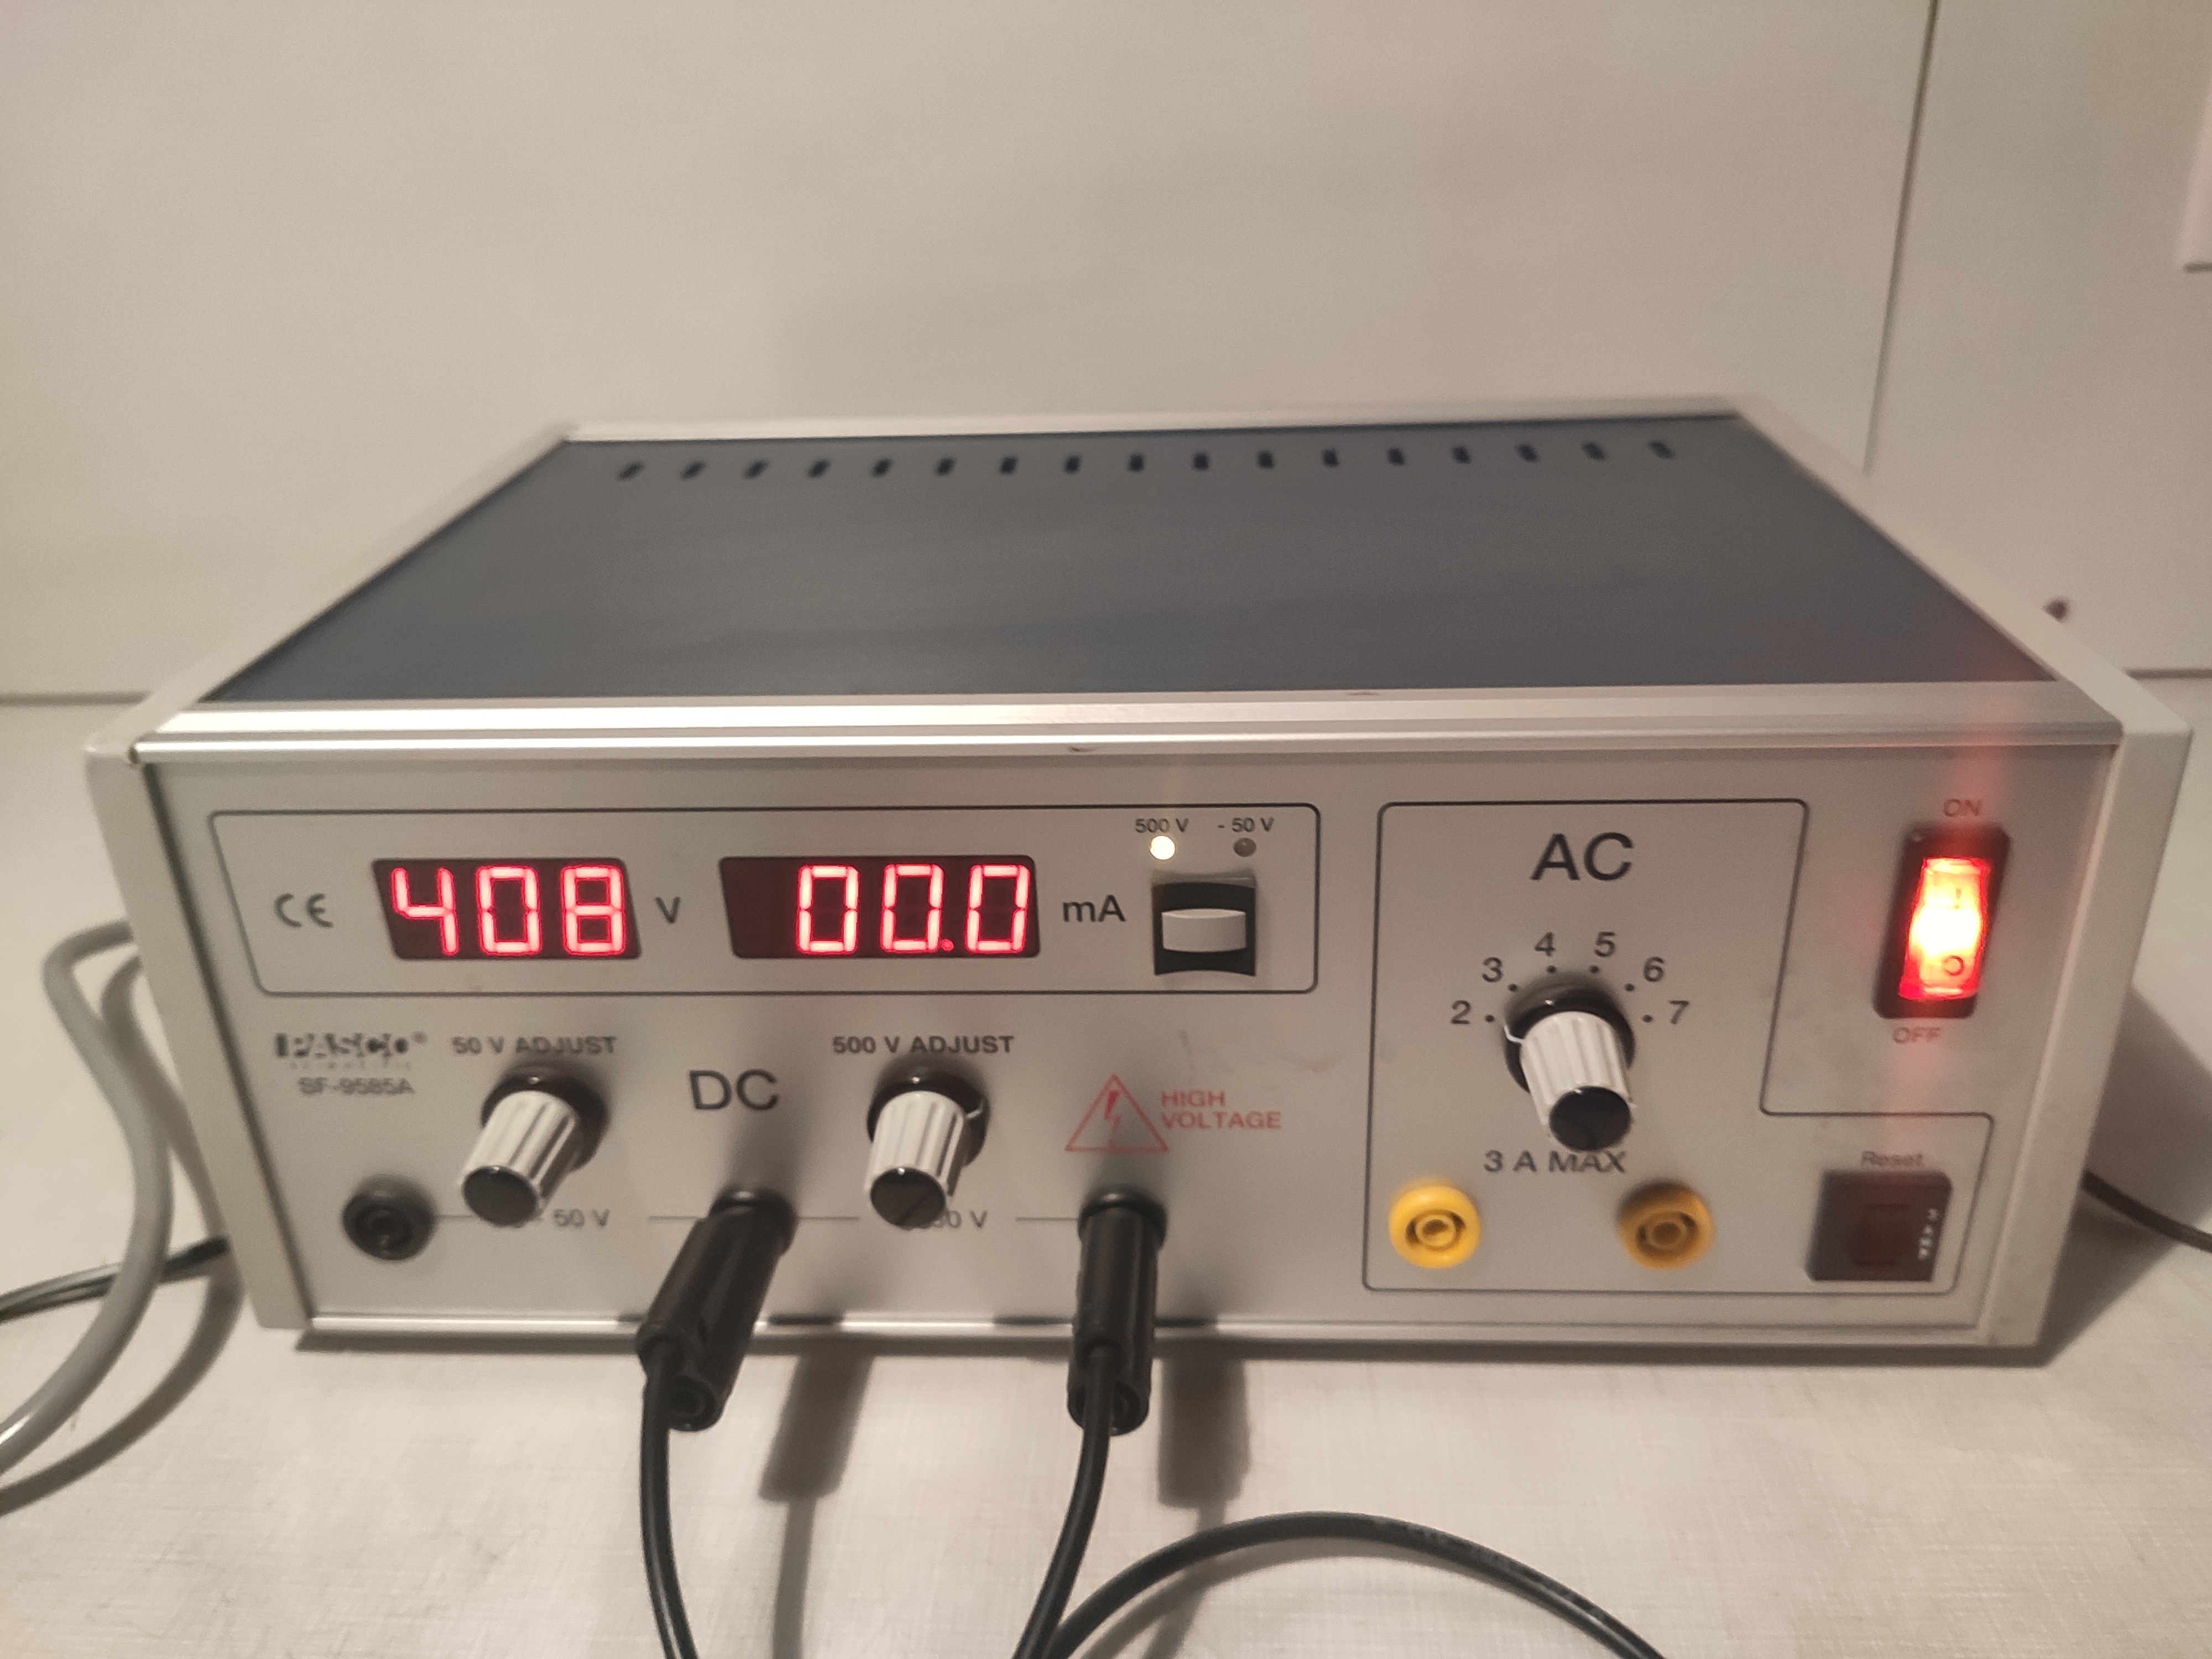
\includegraphics[width=\linewidth]{FotoMillikan2}
    \caption{Prova subfigure}
  \end{subfigure}
  \begin{subfigure}[b]{0.4\linewidth}
    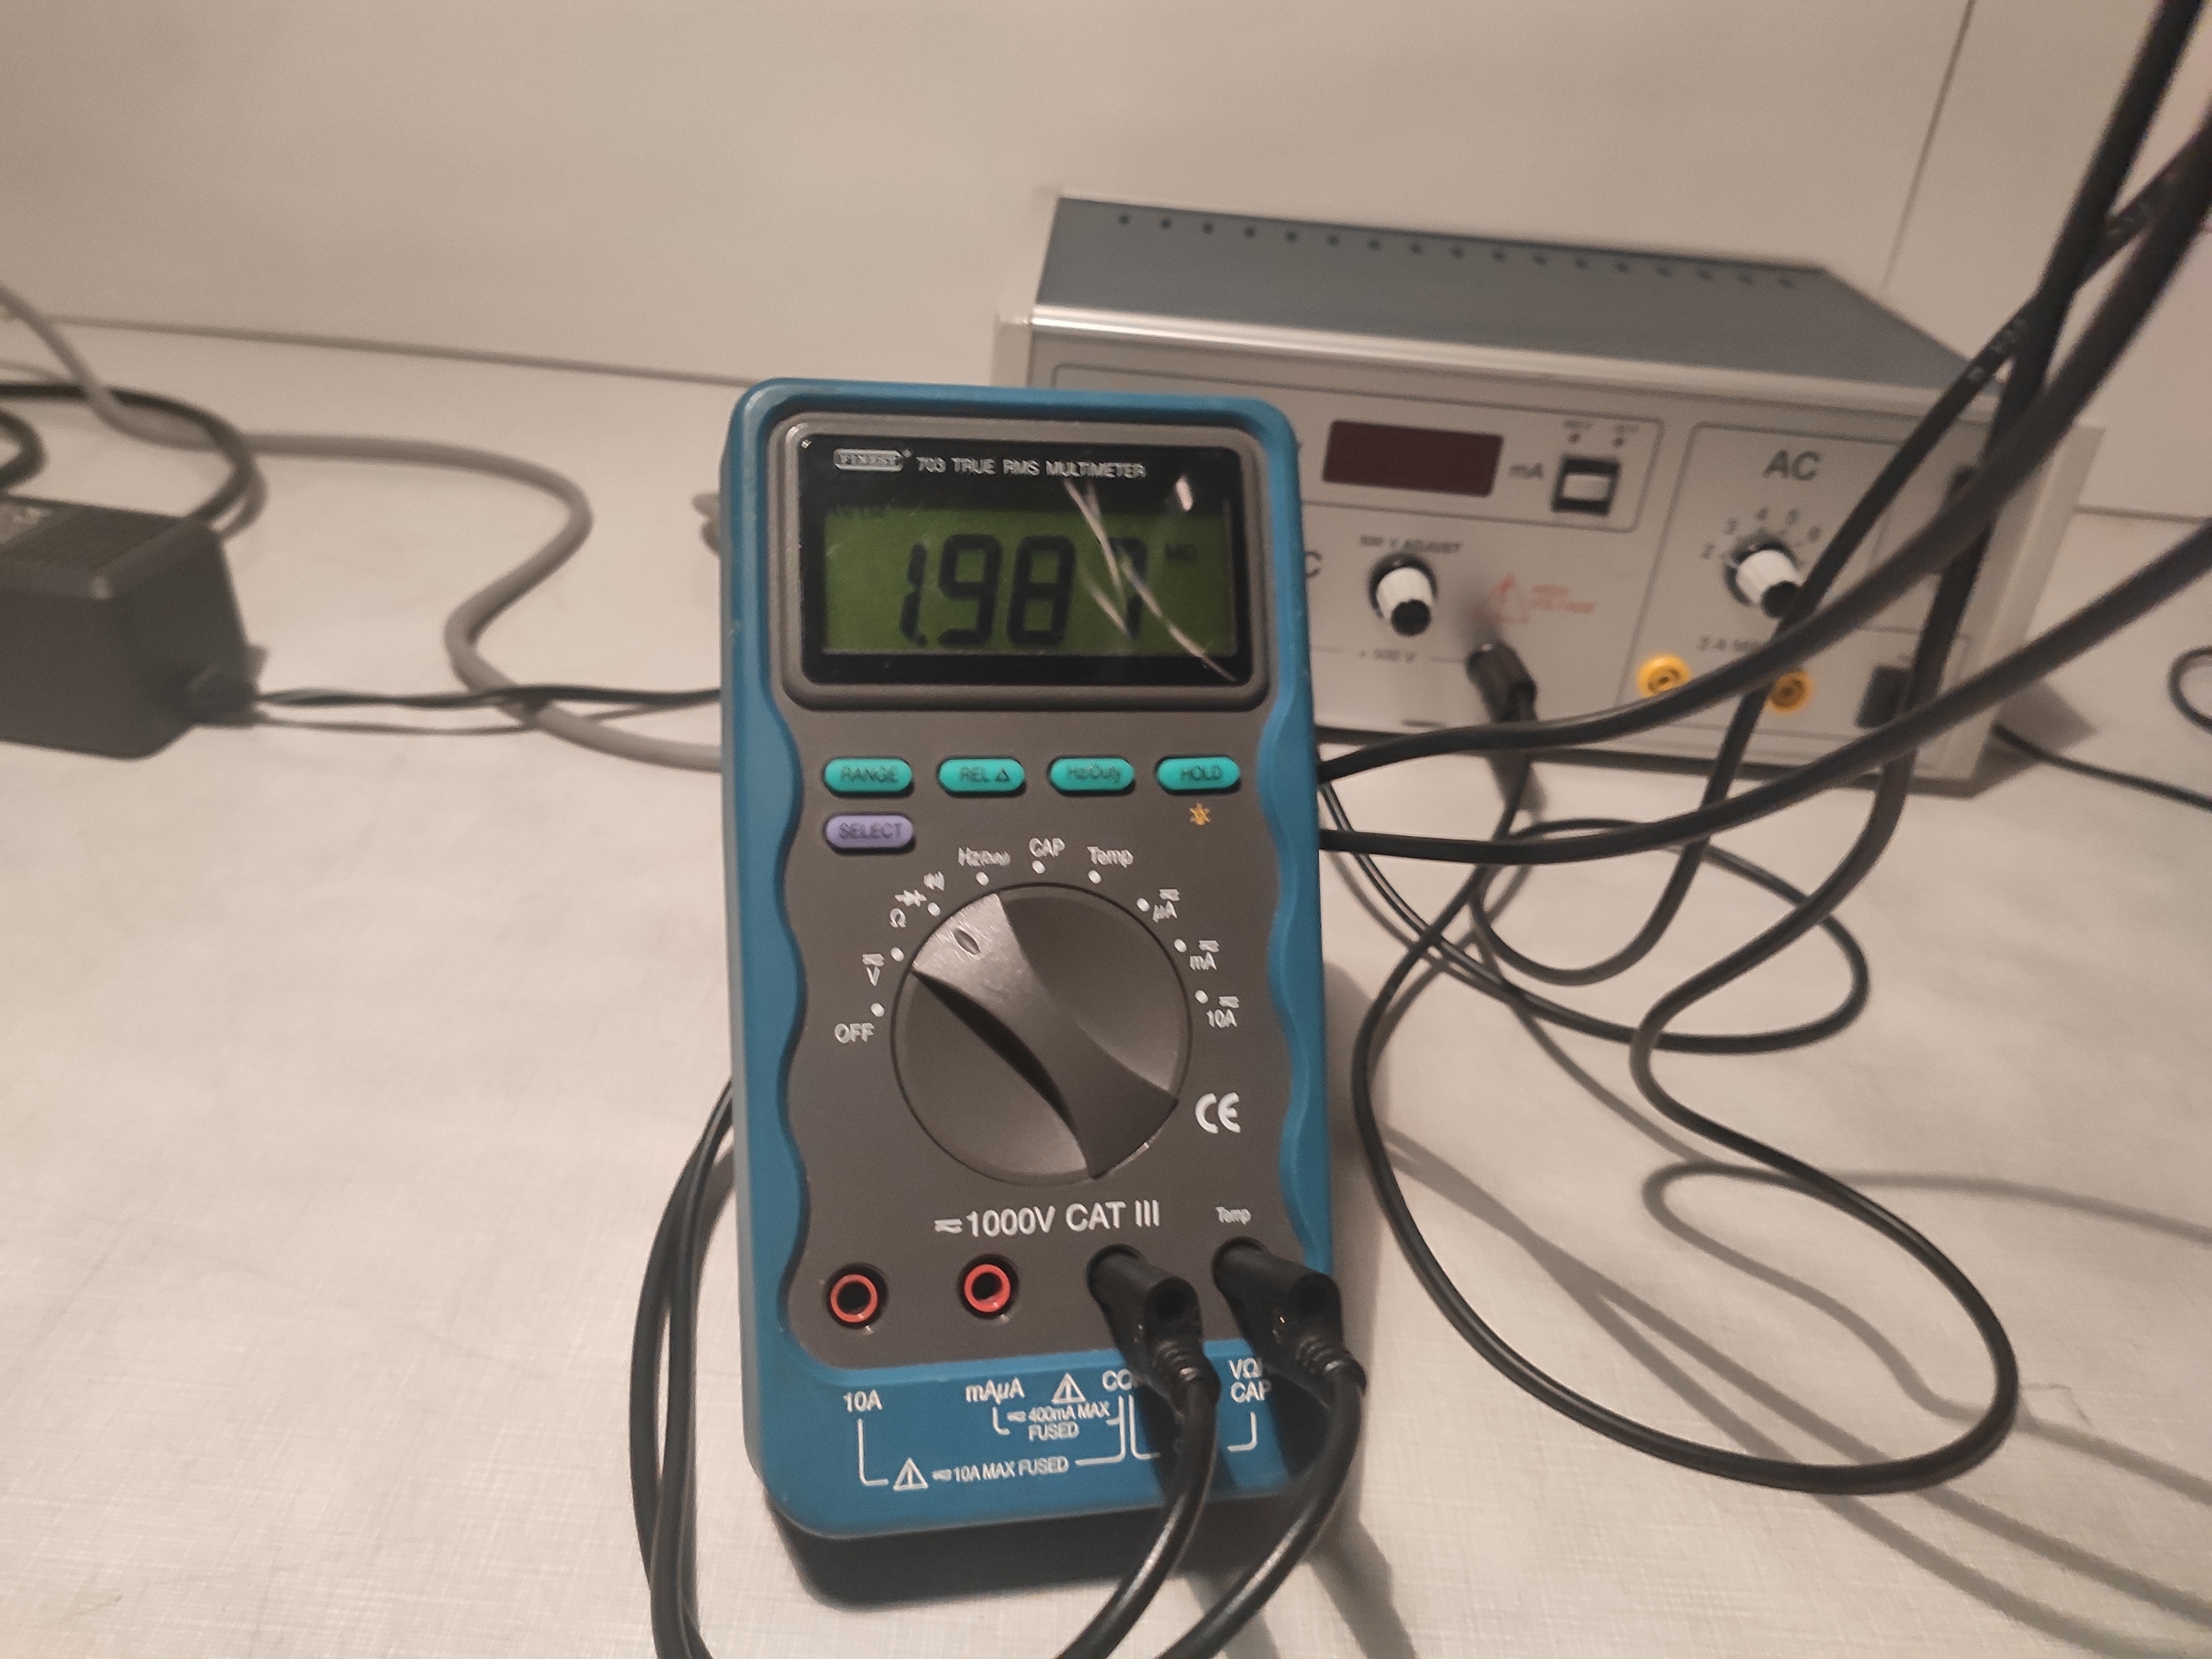
\includegraphics[width=\linewidth]{FotoMillikan3}
    \caption{Foto del termistore}
  \end{subfigure}
\end{figure}

Problemi tecnici riscontrati: 

\section{Misure}

\section{Analisi dei dati}

\section{Conclusioni}
L'esperimento è uscito una merda

\section{}

\end{document}